\section{Literature Review}
% Purpose of this literature review 
This literature review provides a summary on drug resistance in \textit{Mycobacterium tuberculosis} (MTB), focusing on identifying drug resistance-conferring mutations. This review examines mutations conferring resistance, methods for detecting drug resistance, and innovations in these methods. As for scope, this review covers genomic studies using Next-Generation Sequencing (NGS).

Tuberculosis (TB) is an infectious disease primarily affecting the respiratory system  with symptoms including cough with bloody mucus, fever, and fatigue \cite{pai2016}. TB is caused by infection with species in the \mtb-complex (MTBC), a group of closely related bacteria. MTBC includes MTB, the pathogen responsible for human TB, and additional species that infect humans and other animals \cite{gagneux2018}. Generally, MTB is used synonymously with MTBC \cite{riojas2018} due to high genetic similarity among MTBC strains \cite{gagneux2018}. Therefore, this review will refer to the causative agent of TB as \textit{Mycobacterium tuberculosis} or MTB.

TB impacts global significantly with $\sim$ 10 million people being diagnosed in 2022, and is the second leading causes of death (second to COVID-19) with $\sim$ 1.3 million deaths \cite{who2022}. Drug resistance (DR) worsens global anti-TB challenges, as DR renders standard treatments less effective, leading to higher mortality rates and treatment costs \cite{who2022}. Therefore, global and national health programs need to be vigilant with detecting drug resistance in order to inform effective treatment strategies, ultimately mitigating the burden of TB.
\subsection{The Treatment of Tuberculosis and the Critical Role of Detecting Drug Resistance}

Effective treatment against TB is crucial in global efforts, as cases remain high \cite{who2022}. Historically, standard drug treatments have been successful, however, as Multi-Drug resistant TB (MDR-TB) and Extensively Drug Resistant TB (XDR-TB) emerged, they complicated treatment regimens \cite{whitney2016}.  MDR- and XDR-TB demand treatments that more complex, prolonged, and resource-intensive, burdening both patient and provider \cite{whitney2016}. 

\subsubsection{Treatment Regimens for Drug-Susceptible Tuberculosis}
Drug-Susceptible TB (DS-TB) remains the most common form of the disease \cite{who2022}, with well-established treatment regimens \cite{whitney2016}. The standard treatment for DS-TB consists of first-line drugs, and given proper adherence, can effectively resolve TB cases. In addition to TB resolution, appropriate prescription and adherence to DS-TB protocols can prevent drug resistance \cite{whitney2016,islam2017drug,khawbung2021, pai2016}. 

DS-TB treatment lasts about 6 months and involves two phases: an induction phase and a consolidation phase. The induction phase lasts for two months with the following prescribed antibiotics: rifampicin (also called rifampin), isoniazid, pyrazinamide, and ethambutol \cite{horsburgh2015}. The consolidation phase lasts 4 months, where the patient is prescribed rifampicin and isoniazid. In addition, treatments can extend to 9 months if tests still indicate infection after the standard 6-month treatment. Alternatively, shorter treatmets have been developed, where in 2022, the World Health Organisation (WHO) approved a shorter 4-month regimen. This shorter regimen includes 2 months of isoniazid, rifapentine, moxifloxacin , and pyrazinamide, followed by 2 months of rifapentine, moxifloxacin, and pyrazinamide \cite{queensland_health_2023}

Despite the high efficacy of DS-TB treatments, drug-resistance still poses a significant threat to global TB control. Compared to DS-TB, treatments for MDR- and XDR-TB are intricate, costly and drawn-out.

\subsubsection{Treatment Regimens for Drug-Resistant Tuberculosis}
When designing Drug-Resistant TB (DR-TB) treatments, health programs need to introduce an alternative set of drugs.  These drugs are designated as second-line and include new and repurposed compounds \cite{Heyckendorf2018}. Treatments including them are expensive and induces adverse side-effects, making them taxing on the patient, healthcare provider and the national healthcare systems\cite{whitney2016}. 

Drug resistance refers to the ability of MTB to tolerate effects of anti-TB drugs, rendering standard treatments as ineffective \cite{who2022}. Drug resistanceid  classified as: multi-drug-resistant TB (MDR-TB), pre-extensively drug-resistant TB (pre-XDR-TB) and extensively drug-resistant TB (XDR-TB) \cite{Heyckendorf2018,Viney2100361}. MDR-TB is resistant to rifampicin and isoniazid and pre-XDR-TB fulfills the MDR-TB requirements, but is resistant to any fluoroquinolone (FQ).  Lastly, XDR-TB fulfills pre-XDR-TB requirements, but is resistant to any second-line injectable drug (SLID) \cite{Heyckendorf2018,Viney2100361}.

Additional drugs are used to treat MDR-TB, and the WHO categorises them into three groups. Group A includes fluoroquinolones, namely levofloxacin and moxifloxacin, as well as new and repurposed drugs such as bedaquiline and linezolid \cite{Aguilar2023, whoguide2022}. Group B includes newer drugs such as cycloserine and terizidone, and repurposed drugs such as clofazimine. Lastly, Group C includes amikacin/streptomycin (SLIDs), ethambutol, delamanid, pyrazinamide, imipenem-cilastatin/meropenem, ethionamide/prothionamide, and p-aminosalicylic acid \cite{whoguide2022}. These drugs are critical as they form the defense against MDR-TB. 

As recommended by the WHO, treatment for MDR-TB lasts for 18 months, where the WHO recommends a combination of Group A and Group B drugs, with Group C agents used if needed \cite{whoguide2022}. These drugs can impair kidney function, induce liver damage, and trigger cognitive impairments \cite{sturdy2011mdr}. The side effects can call for a different combination of drugs \cite{whitney2016}, further lengthening treatment. 

If a patient harbors an XDR-TB strain, then a more individualised treatment approach that is dependent on the drug susceptibility status of the isolate. The healthcare provider would have develop a treatment regimen from Group A, B and C drugs which lasts for 18 months or longer \cite{who2022,whoguide2022}. 

To tackle the issues of treatment duration and side effects, the WHO has suggested shorter regimens for MDR-TB \cite{whoguide2022}. These treatments are under conditional recommendation, as more clinical trials are conducted\cite{whoguide2022}. The WHO recommends a 6-month regimen for MDT-TB and Pre-XDR-TB, abbreviated as BPaLM (bedaquiline, pretomanid, linezolid 600 mg, moxifloxacin).

Furthermore, a 9-month all-oral regimen has been developed by the WHO and is appropriate for patients with MDR-TB with no observed evidence of FQ resistance. This treatments includes bedaquiline, administered for 6 months, with a blend of FQs (levofloxacin and moxifloxacin), ethionamide, ethambutol, a high dose of isoniazid, pyrazinamide and clofazimine for 4 months. After this 4-month period, if sputum tests are positive, clofazimine should be introduced and the additional blend may be extended to 6 months. Ultimately, the final 5 months will consist of the FQs, clofazimine, ethambutol and pyrazinamide. If ethionamide contraindication is present, e.g. in preganant patients, linezolid (600mg) can be introduced daily for 2 months \cite{whoguide2022}. This all-oral treatment has the added benefit of lowering infection risk and venous thrombosis that occurs during intravenous administration of drugs which require a central long line \cite{whitney2016}. Overall, these newer treatments aim to reduce the adverse side effects of second-line drugs and the burden on the healthcare system.

In conclusion, treatments for both DS-TB and MDR-, Pre-XDR-, and XDR-TB have show success, despite the rising prevalence of drug-resistant cases. However, as treatment regimens become more complex for drug-resistant cases, timely identification of drug resistance is crucial to ensure effective treatment. 

\subsection{Drug Susceptibility Testing for Tuberculosis}
Timely knowledge of drug resistance is essential as it prevents ineffective treatment and inhibits the proliferation of drug-resistant populations in the patient, preventing the patient's condition from worsening. \cite{whitney2016}. Healthcare providers identify the presence of drug-resistance through the process of drug susceptibility testing (DST). DST involves isolating and culturing the patient's samples (usually sputum) and conducting tests to determine which anti-TB agents the sample is resistant or susceptible to. These tests can return a categorical result in the form of a binary, \enquote{resistant} or \enquote{susceptible}, or the result can be numerical in the form of minimum inhibitory concentration (MIC) \cite{whitney2016, islam2017drug}. 

Currently there are three modalities of DST: Phenotypic DST (pDST), Genotypic DST (gDST) and Whole Genome Sequencing DST (WGS-DST) \cite{who2022}. At a surface-level, pDST measures the growth (or lack thereof) of the bacterium in the presence of anti-TB drugs. This is usually a lengthy process, as MTB is slow growing bacilli \cite{gagneux2018}, and is prone to false positives for certain drugs \cite{Yusoof2022}. Therefore, gDST provides much faster and accurate testing by looks for well-known drug-resistance conferring mutations to particular drugs. This process provides a significant cut in DST duration, as it only needs 2 hours to complete.
Despite rapid testing, gDST still suffers from false results as it only screens for well-known resistance markers \cite{whitney2016}. Overcoming this limitation, WGS-DST sequences and evaluates the entire genome to find mutations that confer drug resistance \cite{whitney2016}. This section will discuss the methodology of these 3 DST modalities and their strengths and weaknesses.

\subsubsection{Phenotypic Drug Susceptibility Testing (pDST)}
pDST is the process where drug resistance is indicated by the phenotype of the MTB isolate. If the proportion of growth in the presence of an anti-TB drug exceeds the established critical concentration - the specific concentration of drug where a susceptible MTB isolate's growth would be inhibited - then the isolate is deemed resistant \cite{who2022, who2021tb}. 

There are two ways of conducting pDST: on solid media and liquid media. Solid medium pDST involves growth media such as Löwenstein-Jensen (LJ) or Middlebrook 7H10/7H11 agar. The proportion of growth in the presence of anti-TB drugs suggests resistance, and the turnaround time for results is about 28–42 days \cite{who2022}. Alternatively, liquid medium pDST uses systens such as the Mycobacterial Growth Indicator Tube (MGIT) containing Middlebrook 7H9 liquid media. Systems such as MGIT, rely on proxy measures like fluorescence or chemical changes to ascertain growth and resistance in the presence of anti-TB drugs\cite{Yusoof2022}. Liquid media pDST is than solid media, taking about 14 days, however it is not without it's limitations. pDST is reliable and recommended for first-line drugs, and certain second-line injectables and fluoroquinolones. But MGIT shows high false positive rates for pyrazinamide, demanding specialised lab staff to supervise testing \cite{who2018tb}. 

Although pDST is recommended by the WHO in some cases \cite{whoguide2022}, several limitations prevent its ubiquitous use. The turnaround time is lengthy, delaying critical treatment decisions, and false positives can lead to unnecessary use of expensive second-line drugs, extending treatment and increasing the risk of adverse side effects. Additionally, conducting pDST requires appropriate lab infrastructure and skilled technicians, which is a hurdle in countries with economic challenges, especially since these countries often bear the greatest burden of MTB infections \cite{who_world_bank_2022}.

\subsubsection{Genotypic Drug Susceptibility Testing}

Genotypic Drug Susceptibility Testing (gDST) involves detecting a pre-determined set of resistance-conferring mutations in the MTB isolate. The mutations primarily occur in genes that encode for the targets of anti-TB drugs. For example, to detect resistance to rifampicin, gDST methods focus on identifying mutations in the \textit{rpoB} gene. A common resistance-conferring mutation is S531L, which indicates resistance against rifampicin \cite{sinha2020detection}. 

Tools for gDST include Nucleic Acid Amplification Tests (NAATs) and, less commonly, Line Probe Assays (LPAs). Examples of NAATs include the Xpert MTB/RIF test, which detects both the presence of MTB and rifampicin resistance in about two hours \cite{iram2015rapid}. This is significantly faster than pDST, allowing it to be used in clinical settings, with the major infrastructure needs being constant power supply and provider training \cite{whitney2016}. However, the main issue with gDST is its limited mutation coverage. Tests like Xpert MTB/RIF and LPAs target specific mutations known to confer resistance, potentially missing rare or novel mutations. This can result in false negatives, where gDST fails to detect a resistance-conferring mutation \cite{Yusoof2022}. For example, Xpert MTB/RIF screens for mutations in the rifampicin resistance-determining region (RRDR) -  an 81-bp regions of the \textit{rpoB} gene - where more than 95\% of rifampicin resistance-conferring mutations are detected \cite{rahman2016comparison,musser1995antimicrobial}, this excludes the remainder of the \textit{rpoB} gene.  I491F mutation in the \textit{rpoB} gene associated with drug resistance but is not included in the RRDR \cite{mon2022first}, therefore Xpert MTB/RIF would overlook this mutation, resulting a false negative. To mitigate this, the WHO recommends pDST to be used complementarily to finalise drug susceptibility results \cite{Yusoof2022, whoguide2022}. But the issue with pDST confirmation is that it extends the time required for diagnosis, possibly counteracting the speed advantage of gDST.

\subsubsection{Whole-Genome Sequencing in Drug Susceptibility Testing (WGS-DST)}

WGS-DST overcomes the issue of limited scope and low sensitivity with gDST and the extensive time and resource requirments of pDST, allowing for a comprehensive look into the MTB genome. WGS leverages NGS technologies to sequence the MTB genome entirely and then search for mutations that are associated with drug resistance. Generally,  Illumina WGS experienced more frequent utilisation due to it's higher per-base accuracy \cite{marin2022benchmarking}, however with improvements to long-read sequencing, Nanopore by Oxford Nanopore Technologies (ONT) \cite{hall2023evaluation, smith2020assessing} and PacBio \cite{meehan2018} are becoming more prevalent.

For WGS-DST to occur, patient samples must first be cultured. Following this, library preparation can take place and sequencing can be initiated. Once the isolates have been sequenced, their reads can be mapped to a reference genome,  and for MTB it is the H37Rv reference genome \cite{meehan2018}. Once aligned, the reads will then flow through a variant calling pipeline, to identify genetic variants within the isolate. The specific pipeline is yet to be standardised, and it is a pressing issue as different pipelines can yield different results \cite{walter2020genvar,meehan2018}. 

After completing the WGS sequencing, read mapping and variant calling, a list of variants are produced. With this list and a catalogue containing known mutations associated with drug resistance, the clinician can determine the drug resistance profile of the isolate. This is done by cross-referencing mutations from the variant list with the mutation catalogue. 

In 2021, the WHO published a catalogue including resistant-conferring mutations to 13 anti-TB drugs. This catalogue included a list of MTB mutations that are associated with drug resistance with high confidence, and were developed from using over 40,000 isolates from 46 countries. A lower number of mutations were identified for new and repurposed drugs such as bedaquilline \cite{Walker2022}. This catalogue was updated in 2023 to include data from a larger dataset of isolates and updates mutations for new and repurposed drugs \cite{WHOcatalog}, resulting in the catalogue including mutations for all anti-TB drugs endorsed by the WHO. Ultimately, the WHO catalog is a standardised reference document which lists and describes the confidence of mutations associated with drug resistace and their selection critera \cite{Walker2022,WHOcatalog}. This catalogue also served national TB programs and diagnostic assay manufacturers to develop more accurate DST tools \cite{WHOcatalog}. The scope of the WHO catalogue was deliberately made to be non-exhaustive, as recommendations were only made for mutations with high confidence \cite{Walker2022}.

The main benefits offered by WGS DST is it's ability to comprehensively test for resistance in a wide array of drugs, including variants that are missed by commercial gDST assays \cite{dean202225}. The time needed for WGS-DST ranges from 1 -2 weeks \cite{whitney2016}, being significantly faster than pDST. However, this is slower than the $\sim$ 2 hour turnaround for gDST assays. But, with the cultures available, the sequencing workflow can be optimised to 3-5 days\cite{whitney2016}. Access to WGS technologies is being improved by the development of portable sequencing technologies such MinION developed by ONT, allowing direct testing on sputum samples \cite{hall2023evaluation,smith2020assessing}. 

With the adoption of WGS-DST increasing, widespread implementation is limited by technological and infrastructure needs in low-income regions. Additionally, standardisation in bioinformatic analysis pipelines is highly needed to ensure consistency in DST results across different settings \cite{meehan2018, world2018use, inzaule2021genomic}. 

While, WGS-DST offers a broad window to find novel resistance conferring mutations, it is still affected by incomplete coverage. The process of masking, where sections of the genome are excluded from analysis results in blindspots that are not accounted for when investigating for mutations \cite{modlin2021exact}. This remains a key region for investigation. 

Overall, WGS offers deep and almost exhaustive insight into possible mutations that may cause drug-resistance in Mtb - making it a highly promising modality for widespread DST usage \cite{whitney2016}. This can be improved through innovation in better filters and analysis of previously excluded genomic regions. 
 \subsection{Investigating Mutations in Masked Genomic Regions}
 
\subsubsection{Masking Practices in Mtb Genomic Analysis}

During genomic analysis of the Mtb genome, about 10\% of the Mtb genome commonly needs to be masked \cite{meehan2018}, in a conservative attempt to lower the prevalence of erroneous variant calls. These incorrect calls are a technological limitation of using short-read genome mapping. Short reads (100 - 250bp), are difficult to align to genomic regions that are repetitive or contain homologous sequences \cite{li2008mapping, li2014toward}.  Therefore, the variant caller may identify incorrect mutations, or miss mutations altogether \cite{marin2022benchmarking}. 

These masked regions contain repetitive and homologous sequences, consisting mostly of the \textit{pe/ppe} gene family \cite{marin2022benchmarking}. This gene family, comprised of 168 genes, adopt versatile roles in MTB virulence \cite{gagneux2018,d2023pe}.  As drug-resistant mutation catalogues exclude the masked regions \cite{Walker2022}, investigation into the \textit{pe/ppe} gene family for drug-resistance conferring mutations needs to be conducted. 

\subsubsection{The \textit{pe/ppe} Gene Family and Drug Resistance}

The \ppe gene family proteins contain a conserved \textit{pe} (Proline-Glutamic Acid) or \textit{ppe} (Proline-Proline-Glutamic Acid) motif in their N-terminal domain, with their C-terminal domains being variable, both in sequence and length \cite{d2023pe, cole1998deciphering}. This gene family is over-represented in pathogenic mycobacteria \cite{d2023pe, gagneux2018} and is diverse in function, likely being an adaptation to host's immune system \cite{de2019immune}. 

The \ppe gene family's distribution within the genome is optimised for targeted gene control. Although, the distribution appears as random, the \textit{pe/ppe} genes are packaged into operons consisting of a \textit{pe} gene proceeded by a \textit{ppe} gene \cite{d2023pe, tundup2006clusters}. 

The \textit{pe/ppe} gene family can be characterised their variable C-terminal domains. The PE family can be classified into the PE sub-family and the PE-Polymorphic GC-rich (PE-PGRS) sub-family \cite{cole1998deciphering,gey2006evolution}.  The PE-PGRS sub-family has high GC-content (approximately 80\%), and are highly variable and prone to recombination \cite{gey2006evolution, daleke2012general}. The PPE family can also be classified into two subfamilies, namely the PPE and PPE-Major Polymorphic Tandem Repeat (PPE-MPTR) \cite{cole1998deciphering,gey2006evolution}. The PPE-MPTR sub-family proteins have been observed to be exceptionally large, with secreted proteins exceeding 3000 amino acids in length \cite{hermans1992characterization,cole1998deciphering, gey2006evolution}. 

The \ppe gene family are also involved in antibiotic resistance \cite{d2023pe}. Mutations within \ppe regions have are associated with drug resistance, specifically through the action of gene-pair mutations. A pair of genes, consisting of a gene encoding a drug target and a \ppe gene are associated in a drug-resistant isolate \cite{d2023pe}. Examples include \textit{KatG-PPE54}, where mutations in both \textit{KatG}, whose gene product activates isoniazid \cite{islam2017drug} and \textit{PPE54} were observed in isoniazid resistant isolates. Likewise, another gene pair was \textit{rpoB} (encodes drug target for rifampicin \cite{islam2017drug}) and \textit{PPE-54} were observed in a rifampicin-resistant isolate. Other gene pairs were observed for common anti-TB drugs such as ethambutol and streptomycin \cite{cui2016bioinformatics}. Therefore genes in the \ppe gene family are prime targets for investigation. 

Aside from gene-pair interactions, mutations in certain sub-families have been shown to be enriched in resistant isolates. Specifically, numerous members of the PE-PGRS sub-family were observed in XDR-TB isolates \cite{kanji2015characterization}.  Moreover, mutations in PPE genes were  associated with an expansion in Isoniazid resistance \cite{hang2019whole}.

Additionally, \ppe proteins alter MTB cell functioning, rendering them resistant to anti-TB drugs. For example, PE11, a protein with esterase activity is involved with cell wall remodelling, increasing the hydrophobicity of the cell surface and its impermeability to anti-TB drugs \cite{singh2016pe11}.

Currently, genes in the \ppe family are commonly masked in standard analyses, meaning potential drug resistance-conferring mutations may be overlooked, motivating changes to standard masking practices. This will accommodate the discovery of newer mutations, thus improving mutation catalogue accuracy. 

\subsection{Re-evaluating the Masking Approach}

Masking involves excluding regions of the MTB genome, as they are comprised of repetitive, highly homologous and GC-rich regions, rendering them difficult to analyse (Figure 2). These regions can lead to fluctuations in coverage due to reads mapping to multiple locations which may misinterpreted as deletions. 

Masked regions of the genome contain the \ppe gene family, sequences homologous to other regions of the genome and mobile genetic elements \cite{meehan2018,marin2022benchmarking,modlin2021exact}. As a result, their exclusion comes at a cost of missed alignments, causing potentially missed drug-resistance conferring mutations. Specifically the exclusion of the \ppe gene family is costly, due to mutations in those regions, as mentioned previously, have been associated with drug-resistance \cite{cui2016bioinformatics, kanji2015characterization} and they are integral to MTB virulence \cite{d2023pe}.  Therefore, this motivates the need for more accurate and concentrated masking practices. 

\begin{figure}
    \centering
    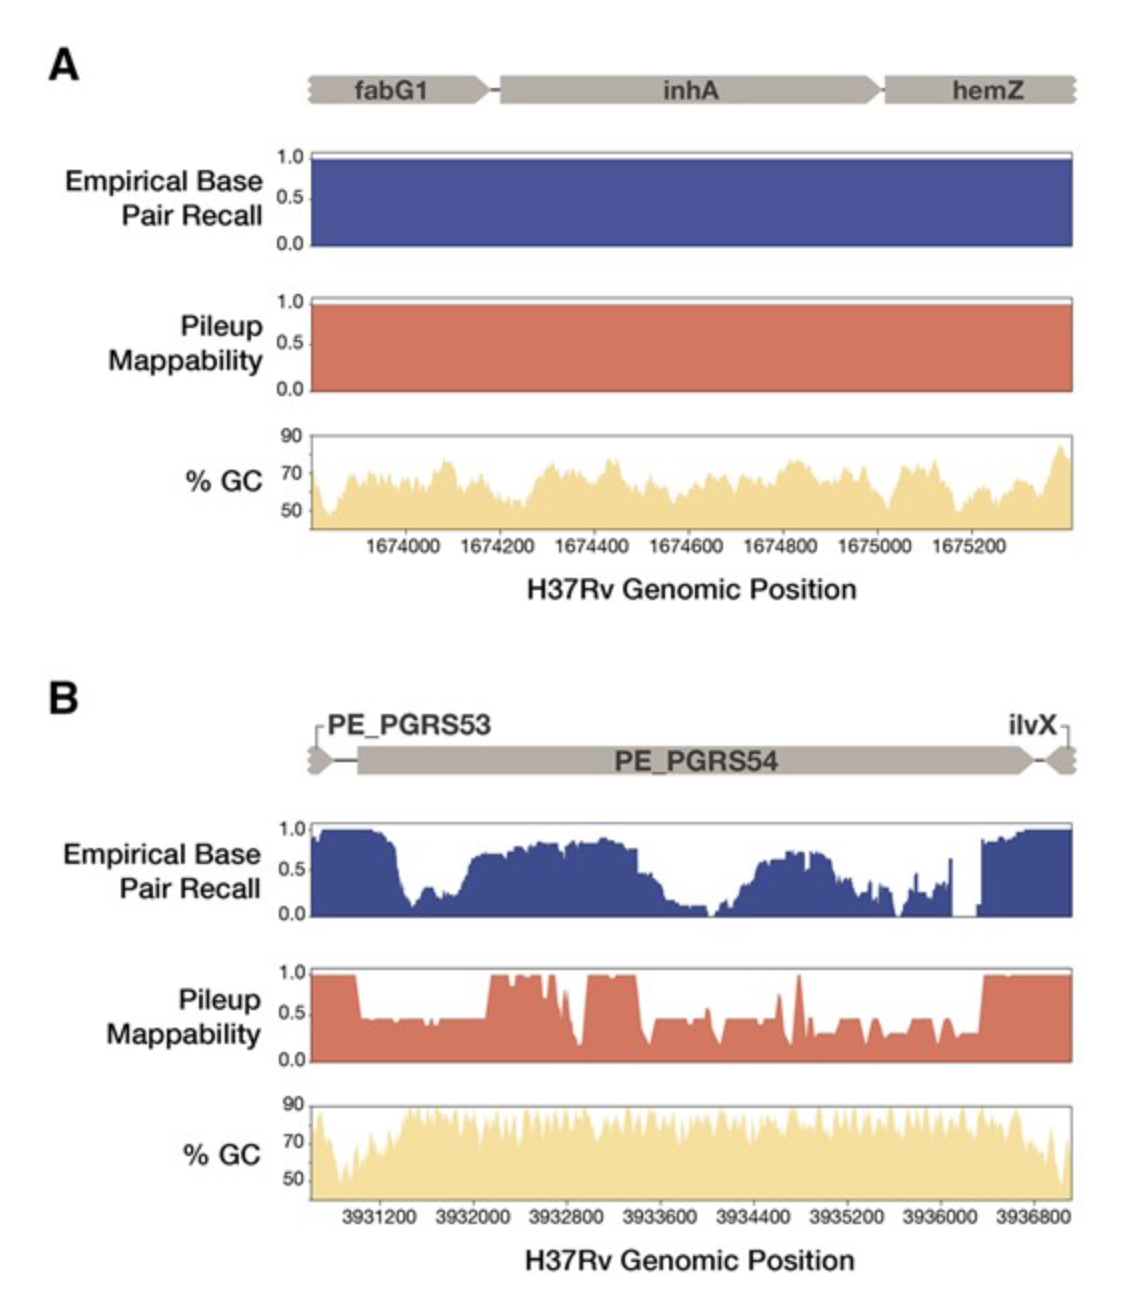
\includegraphics[width=0.5\linewidth]{figures/Screen Shot 2024-11-01 at 5.22.47 am.png}
  \caption{Comparison of empirical base pair recall (EBR), pileup mappability, and GC content across selected regions of the H37Rv MTB genome. (A) Shows the region including \textit{fabG1}, \textit{inhA}, and \textit{hemZ}, which has high EBR and mappability. (B) Shows a region containing \textit{PE\_PGRS53} and \textit{PE\_PGRS54}, illustrating the lower empirical recall and mappability (Marin \etal, 2022).}
    \label{fig:enter-label}
\end{figure}

Empirical studies investigating the efficacy of conservative masks has supported the need for newer masking regimes. A benchmarking study by Marin \etal, found that approximately 90\% of all false positive variant calls occurred in only a 65kb sliver of the MTB genome when no masking is applied \cite{marin2022benchmarking}. This represents about 1.5\% of the MTB genome, and comparing that to the 10\% traditionally masked highlights the unnecessary exclusion of highly mappable regions. Reinforcing this, Modlin et al., found that low-coverage regions, or  \enquote{blind spots} were less prevalent in previously masked regions, while paradoxically, many of these blind spots were identified in regions that had been included in analyses \cite{modlin2021exact}. These studies also discovered that the \ppe gene family could be analysed with the use of newer masks. Marin et al., reported that 52/168 or about one-third of \ppe genes had high mappability, although the sub-families PE-PGRS and PPE-MPTR showed lower mappability \cite{marin2022benchmarking}. Moreover, Modlin \etal reported the distribution of blind spots were lower than expected in \ppe regions and that certain \ppe genes do not have any blind spots \cite{modlin2021exact}. 

\begin{figure}
    \centering
    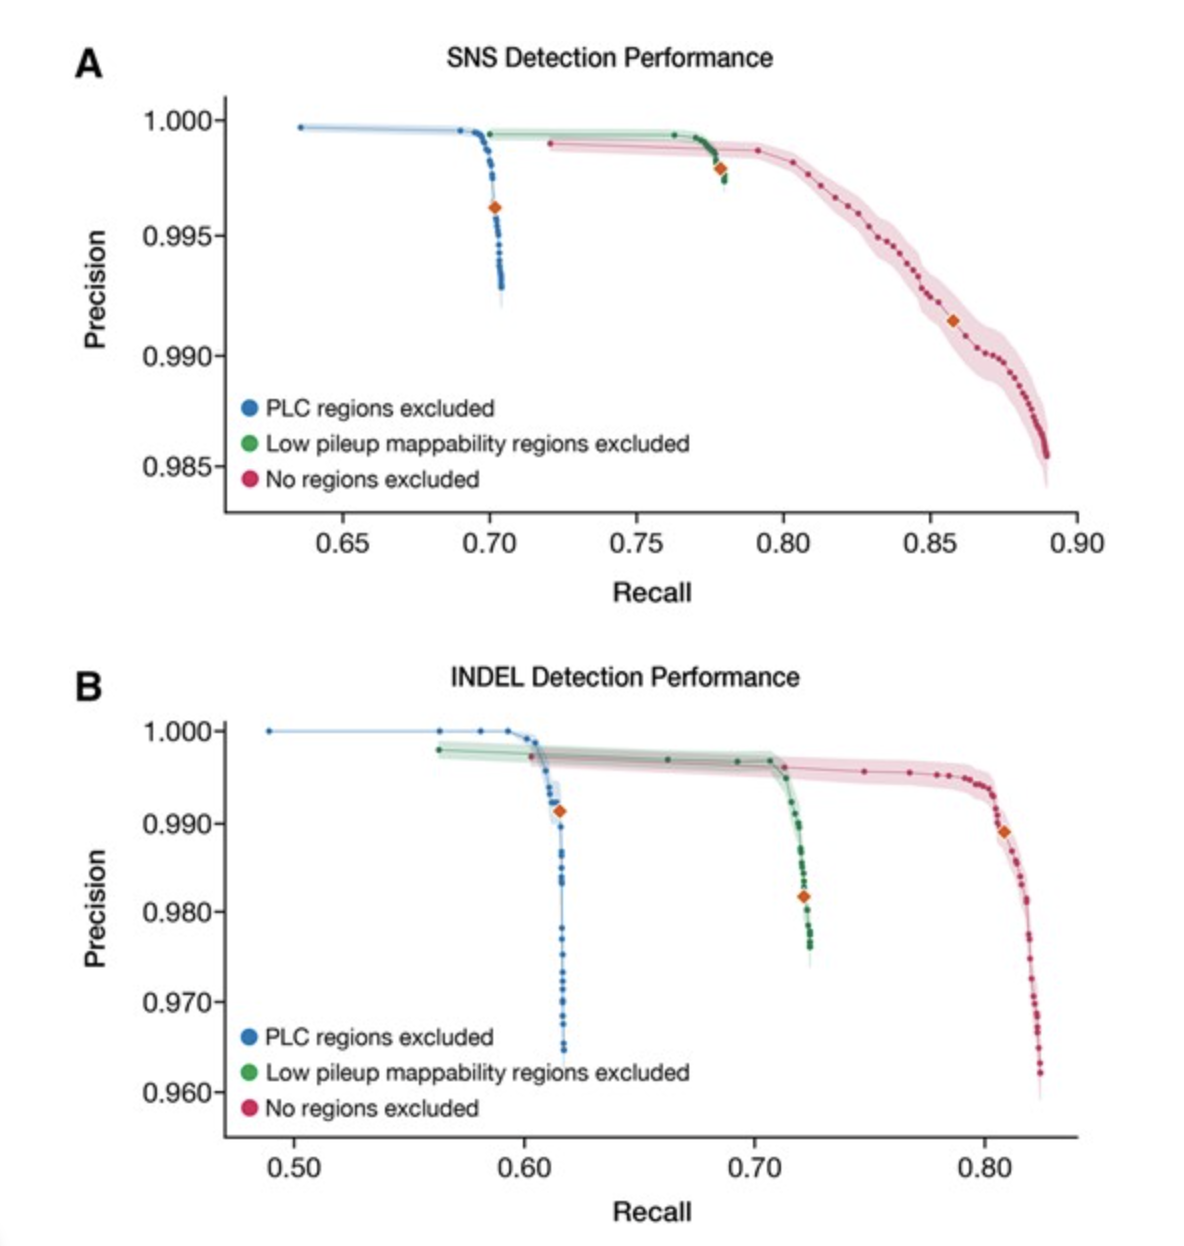
\includegraphics[width=0.5\linewidth]{figures/Screen Shot 2024-11-01 at 5.26.51 am.png}
    \caption{Mean single nucleotide substitution (SNS) and INDEL variant calling approaches across different masks. (A) SNS detection performance was assesed with three masking strategies: permissive masks (low pileup mappability regions excluded), no masking (no regions excluded) and traditional masks (PLC regions excluded). (B) Short INDEL performance was also included. The orange diamonds represent mean precision and recall at MQ threshold of 40. (Marin \etal, 2022) }
    \label{fig:enter-label}
\end{figure}

Establishing the importance of revised masking practices and the need to analyse \ppe genes, newer masking protocols have been developed. Firstly, Marin \etal intended to refine currently excluded regions, labelling them as \enquote{Refined Low-Confidence} (RLC) regions. RLC regions span only about 4\% of the genome, in contrast to the 10\% that are usually masked. This mask was developed through optimisation of certain metrics used in variant calling. Marin \etal focused on Mapping Quality (MQ), which measure the probability that a read was incorrectly aligned to the reference genome. By optimising the threshold for MQ, Marin \etal, were able to significantly reduce the size of the excluded regions whilst maintaing precision without sacrificing recall (Figure 3) \cite{marin2022benchmarking}. In addition, Modlin \etal had bench-marked different sequencing workflows used by Illumina WGS, and analysed the distribution of blind-spots across the genome. As a result providing more accurate masks \cite{modlin2021exact}. 

Accurate masking enables detailed insight into previously masked genomic regions, especially the regions accomodating the \ppe gene family. This will facilitate thorough investigation in regions previously ignored for resistance-conferring mutations. These mutations may potentially explain drug-resistant phenotypes that do not have an associated mutation, or it may predict drug resistance in other cases. Thus, prospective genotype-phenotype associations developed from applying newer masks can provide meaningful contributions to mutation catalogues, ultimately enhancing drug-resistance detection and treatment of drug-resistant tuberculosis.  







